%%%%%%%%%%%%%%%%%%%%%%%%%%%%%%%%%%%%%%%%%%%%%%%%%%%%%%%%%%%%%%%%%%%
%                                                                 %
%  GEANT manual in LaTeX form                                     %
%                                                                 %
%  Michel Goossens (for translation into LaTeX)                   %
%  Version 1.00                                                   %
%  Last Mod. Jan 24 1991  1300   MG + IB                          %
%                                                                 %
%%%%%%%%%%%%%%%%%%%%%%%%%%%%%%%%%%%%%%%%%%%%%%%%%%%%%%%%%%%%%%%%%%%
\Documentation{R.Brun, F.Bruyant}   
\Submitted{01.10.84}           \Revised{26.10.93}
\Version{Geant 3.16}           \Routid{BASE090}
\Makehead{The reference systems and physical units}
\section{The {\tt MA}ster {\tt R}eference {\tt S}ystem ({\tt MARS})}
 
The kinematic variables of the particles transporter by {\tt GEANT}
are always referred to the so-called 
{\tt MA}ster {\tt R}eference {\tt S}ystem ({\tt MARS}). This system
is implicitly defined as the local reference system of the first
volume defined, which contains all the others. This is a Cartesian
coordinate system with axis $\hat{x}, \hat{y}, \hat{z}$ where
$\hat{z} = \hat{x} \times \hat{y}$.
If the axes are labelled {\tt (X,Y,Z)}, then the point {\tt P}
is represented in fig \ref{fg:base090-1}.
 
\begin{figure}[hbt]
      \centering
      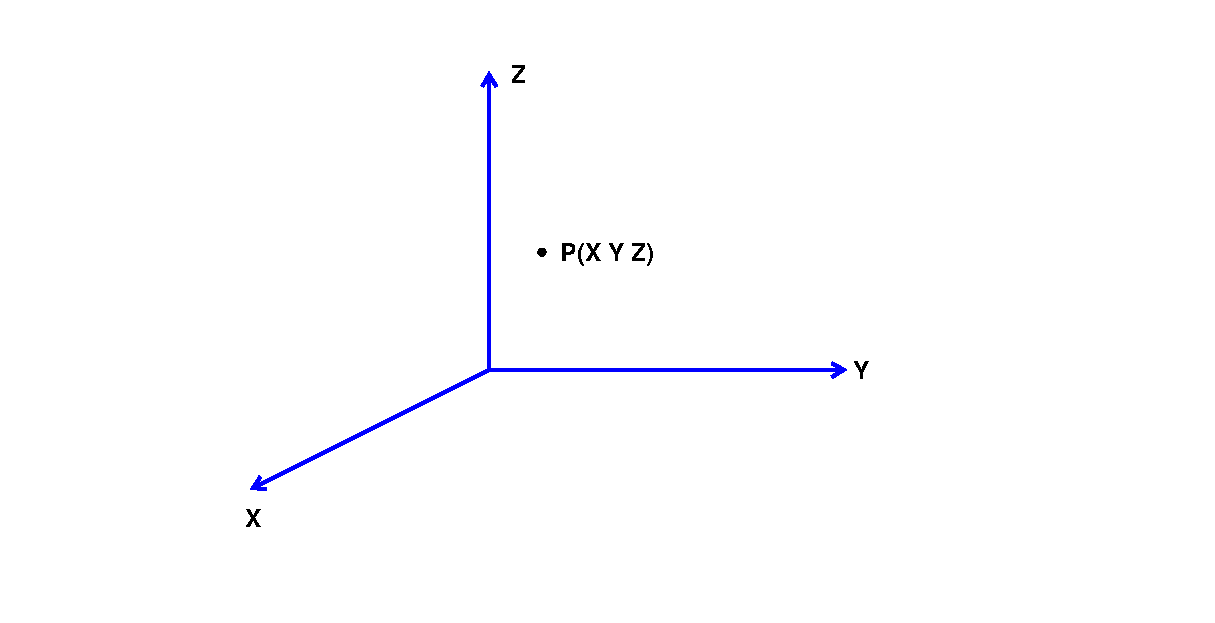
\epsfig{file=eps/base090-1.eps,width=10cm}
      \caption{{\tt GEANT} reference system}
      \label{fg:base090-1}
\end{figure}

Tracking is performed in the {\tt MARS} and the input position for
user routines such as the magnetic field routine is given in this
system.

\section{The local reference systems ({\tt MRS} and {\tt DRS})}
 
As explained in {\tt [GEOM001]}, the setup is
described via the definition of an initial volume inside which all
the others will be positioned. In {\tt GEANT} terminology, each time
a volume has contents, created either via division or by positioning 
other volumes inside, it is called a {\tt MOTHER}. The volumes contained
are called {\tt DAUGHTER}s, and they, in turn, can contain volumes to
a depth of 15 levels. This is sometimes referred to as a {\it Russian doll}
geometry.
 
Every volume defined in {\tt GEANT} has a reference system attached to
it (see {\tt GEOM} section). When this volume has contents, this
is referred to as the {\tt M}other {\tt R}eference {\tt S}ystem
({\tt MRS}, with origin in O$_m$). Daughters
are positioned inside the mother with respect to the {\tt MRS}. The 
{\tt MRS} of the first volume defined, containing all the others, is
nothing else than the {\tt MARS}.

Each one of the daughters has its own reference system, which is referred
to as the {\tt D}aughter {\tt R}eference {\tt S}ystem, or {\tt DRS} with
origin in O$_d$. 

The transformation of a point from the {\tt MRS} (V$_m$)
to the {\tt DRS} (V$_d$), at any level, is performed using a rotation 
matrix $[R]$ and a translation vector $T$ via the relation :
     \[ V_d  =[ R ](V_m -T) \]
The components of $T$ are the projections of the vector  $ (O_m, O_d) $
onto the {\tt MRS} axes.
The rotation matrices are computed from
the spherical angles of each of the axes of the
daughter reference systems ({\tt I, II, III})
with respect to the mother reference system ({\tt 1, 2, 3}).
The spherical angles $\Theta$ and $\Phi$ of a
direction $D$ are defined as follows :
\begin{DLtt}{MMMMM}
\item[$\Theta$]     is the angle formed by the axis 3 and D
                 ($0^{\circ}\;<\;\Theta\;<\;180^{\circ}$).
\item[$\Phi$]      is the angle formed by the axis 1 and the projection
                of D onto the plane defined by the axes 1 and 2
                 ($0^{\circ}\;<\;\Phi\;<\;360^{\circ}$).
\end{DLtt}
Examples are given in {\tt [GEOM200]}.
The various rotation matrices required for a given setup must be
defined by the user during the initialisation stage.
A number is assigned to each matrix {\tt [GEOM200]}.
The translation vector and the number of the rotation
matrix are specified by the user when the volumes are
positioned inside their mother {\tt [GEOM110]}.

\section{Physical units}
 
Unless otherwise specified, the following units are
used throughout the program:
centimeter, second, kilogauss, GeV, GeV c$^{-1}$ (momentum), 
GeV c$^{-2}$ (mass) and degree.
